tion\documentclass[8pt]{article}
\usepackage{amssymb}
\usepackage{babel}
\usepackage{geometry}
\usepackage{amsmath}
\usepackage{amsthm}
\usepackage{framed}
\usepackage{pifont}
\usepackage{listings}
\usepackage{tikz}
\usepackage{hyperref}
\usepackage{float}
\usepackage{paralist}
\usepackage{xcolor}
\usepackage{tikz}
\usepackage{booktabs} 
\usepackage{siunitx} 
\usepackage{pdflscape}
\usepackage{tabularx} % For tables with adjustable-width columns
\usepackage{lipsum} 
\usepackage{geometry}

\usetikzlibrary{automata, positioning, arrows}

\sisetup{
  round-mode          = places, % Rounds numbers
  round-precision     = 4, % to 4 places
  scientific-notation = true % Use scientific notation
}


\def\ra{\rightarrow}
\def\rr{\Rightarrow}
\def\tf{$\Rightarrow$}
\def\oo{\infty}
\def\l/{\backslash}
\def\0{\emptyset}
\def\P{\mathbb{P}}
\def\px{\mathcal{P}_X}
\def\s{\mathcal{S}}
\def\a{\mathcal{A}}
\def\bs{\mathcal{B}}
\def\lm{\mathcal{L}}
\def\R{\mathbb{R}}
\def\E{\mathbb{E}}
\def\Z{\mathbb{Z}}
\def\m{\mathcal{M}}
\def\N{\mathcal{N}}
\def\b{\,\,\,}
\def\activity{\textit{activity} }
\def\down{\textit{down\_event} }
\def\up{\textit{up\_event} }
\def\textchange{\textit{text\_change} }
\def\cursor{\textit{cursor\_position} }
\def\wordcount{\textit{word\_count} }
\def\id{\textit{id} }
\def\eventid{\textit{event\_id} }
\def\downtime{\textit{down\_time} }
\def\uptime{\textit{up\_time} }
\def\actiontime{\textit{action\_time} }
\def\Input{\textit{Input} }
\def\Nonproduction{\textit{Nonproduction} }
\def\Remove{\textit{Remove/Cut} }
\def\Paste{\textit{Paste} }
\def\Replace{\textit{Replace} }
\def\MoveFromTo{\textit{Move From To} }



\title{STAT 432 Final Project}
\author{Ruiming Min(rmin4), Zixuan Fan(zixuanf5), Yewen Li(yewenli2)}
\date{\today}

\begin{document}

\maketitle

\section{Project Description and Summary}

\section{Literature Review}
On the Kaggle website, there are many discussions with profound quality and insightful materials. 
In general, participants tend to use the modern deep learning models such as convolution neural network,
transformer model etc. The classical statistical learning models do not prove to be effective in this competition. 
Potential reasons for this phenomenon are that the classical models are not able to capture the complex patterns in the data. 
The writing style of the text does not follow any explicit linear or quadratic patterns. 
For this reason, the regression models, which is based on the linear assumption, are not able to capture the patterns in the data.
On the other hand, the classification models, also makes assumptions on the distribution of data in certain clusters, 
while the distribution of the handwriting data is highly dependent on our data processing. 
Thus, the classification models may not be effective, either, because some patterns are either lost in processing or cannot be summarized into single 
record for each observation. 

Looking into various discussions, we found two revealed methods highly effective with detailed descriptions. 
We analyze those methods and exploit some features in our project. 
\subsection{LGBM Regression}
\href{https://www.kaggle.com/code/hengzheng/link-writing-simple-lgbm-baseline}{Link Writing Simple LGBM baseline} by ZhengHeng
presented the author's Python implementation of LGBM regression model for score prediction. The author's approach 
reached a score of 0.589 and ranked 382nd on the leaderboard. Although the author was not amongst the top of the leaderboard, 
his approach was simple and inspired many other people, as shown in this \href{https://www.kaggle.com/competitions/linking-writing-processes-to-writing-quality/discussion/451081}{discussion}.

ZhengHeng's approach can be summarized into two steps. First, he did a feature engineering on the data. 
By considering the physical meaning of the relationship between features, he generated some new features from 
the existing log and discarded those high correlated features. Some of new features are the ratio of 
\textbf{word count}, \textbf{idle time} and \textbf{event time}. Second, he trained the LGBM regression model
on a five-fold cross validation. The Light Gradient Boosting Machine (LGBM) is a gradient boosting framework
that uses tree based learning algorithms. 
This newly developed model grows tree vertically in a leaf-wise fashion, while the traditional tree-based models
grow horizontally in a level-wise fashion. The author tuned the model manually and publish the best parameters. 
% Decide if we want to use this regressor?

\subsection{Feature Engineering}
\href{https://www.kaggle.com/code/hiarsl/feature-engineering-sentence-paragraph-features}{Feature Engineering Sentence and Pargraph Feature} by Matthias Hauser
gives us a detailed description of feature engineering based on the nature of the training dataset and also the mean importance of its variables. Based on the author's feature engineering,
the author improved his score to 0.586 and ranked 54th on the leaderboard. Also, this post got a gold medal in the notebook competition. As one of the highest-ranked notebooks, 
his work is very valuable and worth learning from. There are also many discussions about this notebook, which is shown in this \href{https://www.kaggle.com/code/hiarsl/feature-engineering-sentence-paragraph-features/comments}{discussion}.

Matthias Hauser's work can be summarized into three groups: \textbf{sentence features, paragraph features and other features}. 
For sentence features, the author used the average length of sentences, the number of sentences, and so on. 
For paragraph features, the author used the average length of paragraphs, the length of the first paragraph, the number of paragraphs and so on.
For other features, the author used the average length of words, the number of words, pause time, and so on.
These features are very useful and meaningful which could be used in our project. Moreover, the author's work gives us a good implementation of feature engineering.

Futhermore, the author also gave us the mean importance of his variables. The graph is shown at the end of \href{https://www.kaggle.com/code/hiarsl/feature-engineering-sentence-paragraph-features/notebook}{his post}.
The importance of his variables shows that the importance of his variables is very close to our natural knowledge. Some of the most important variables are \textbf{the length of words}, \textbf{pause time}, and \textbf{sentence length}, which are also the standard by which we judge a person’s writing level in life.
Based on his work, we could do more feature engineering like delete ratio, text change ratio, and paragraph balance, to improve our score.

\section{Data processing}
Based on \href{https://www.kaggle.com/competitions/linking-writing-processes-to-writing-quality/data}{the structure of the data on Kagge}, each indevidual is represented by a sequence of events and each event has plenty of variables.
The variables include the following:
{
\small
\begin{compactitem}
    \item \textbf{\textit{id}} - The unique ID of the essay.
    \item \textbf{\textit{event\_id}} - The index of the event, ordered chronologically.
    \item \textbf{\textit{down\_time}} - The time of the down event in milliseconds.
    \item \textbf{\textit{up\_time}} - The time of the up event in milliseconds.
    \item \textbf{\textit{action\_time}} - The duration of the event (the difference between down\_time and up\_time).
    \item \textbf{\textit{activity}} - The category of activity which the event belongs to.
    \begin{compactitem}
        \item \textit{Nonproduction} - The event does not alter the text in any way.
        \item \textit{Input} - The event adds text to the essay.
        \item \textit{Remove/Cut} - The event removes text from the essay.
        \item \textit{Paste} - The event changes the text through a paste input.
        \item \textit{Replace} - The event replaces a section of text with another string.
        \item \textit{Move From} \([x1, y1]\) To \([x2, y2]\) - The event moves a section of text spanning character index \(x1, y1\) to a new location \(x2, y2\).
    \end{compactitem}
    \item \textbf{\textit{down\_event}} - The name of the event when the key/mouse is pressed.
    \item \textbf{\textit{up\_event}} - The name of the event when the key/mouse is released.
    \item \textbf{\textit{text\_change}} - The text that changed as a result of the event (if any).
    \item \textbf{\textit{cursor\_position}} - The character index of the text cursor after the event.
    \item \textbf{\textit{word\_count}} - The word count of the essay after the event.
\end{compactitem}
}

This would make the data very sparse and hard to process.
Especially, those non-numeric variables like \activity are hard to directly use in the model. 
Therefore, in this project, effective data processing will be a crucial component and will significantly impact future outcomes.
To achieve better data processing results, the data processing in this project can be broadly divided into three parts: \textbf{data integration}, \textbf{feature engineering}, and \textbf{dimensionality reduction}.

\subsection{Data Integration}
In order to integrate the data, getting the whole text of each individual's essay is the first step.
Based on the data structure, follwoing the \eventid and the instructions of \activity, we designed a algorithm to get the whole text of each individual's essay.

Also, the complicated construction of the \activity makes the directly use of it impossible. To summarize and integrate it, we designed a algorithm to get the \textbf{total number} of each \activity.
Besides, from the basic understanding of the quality of writing, the writing style of the text also plays an important role in the quality of writing.
Therefore, we designed a algorithm to get the whole number of each indeviduals' \textbf{total number} of change their activity.

After dealing with the \activity and its related variables (\down , \up , \textchange , \cursor , and \wordcount), we also need to deal with \downtime , \uptime , and \actiontime . 
For \actiontime , there are three obviously essential indexs: \textbf{mean}, \textbf{variance}, and \textbf{sum}.
However, since downtime and \uptime contain the informatin of the time point insteade of a interval, the situation is a little bit different. 
According to the concept of writing skill, thinking time is an important variable.
Therefore, we designed a algorithm to get the sequnece of \textit{pause\_time}, which is the difference between the \up of the previous event and the \down of the next event.
Then, same as the \actiontime , we get the \textbf{mean}, \textbf{variance}, and \textbf{sum} of the \textit{pause\_time}.

% To summarize the data integration, we get the following variables:

%{
%\small
%\begin{compactitem}
%    \item \textbf{\textit{id}} - The unique ID of the essay.
%    \item \textbf{\text{essay\_text}} - The whole text of the essay.
%    \item \textbf{\textit{num\_nonproduction}} - The total number of \textit{Nonproduction} activity.
%    \item \textbf{\textit{num\_input}} - The total number of \textit{Input} activity.
%    \item \textbf{\textit{num\_remove}} - The total number of \textit{Remove/Cut} activity.
%    \item \textbf{\textit{num\_paste}} - The total number of \textit{Paste} activity.
%    \item \textbf{\textit{num\_replace}} - The total number of \textit{Replace} activity.
%    \item \textbf{\textit{num\_move}} - The total number of \textit{Move From To} activity.
%    \item \textbf{\textit{num\_change\_activity}} - The total number of change activity.
%    \item \textbf{\textit{mean\_action\_time}} - The mean of \textit{action\_time}.
%    \item \textbf{\textit{var\_action\_time}} - The variance of \textit{action\_time}.
%    \item \textbf{\textit{sum\_action\_time}} - The sum of \textit{action\_time}.
%    \item \textbf{\textit{mean\_pause\_time}} - The mean of \textit{pause\_time}.
%    \item \textbf{\textit{var\_pause\_time}} - The variance of \textit{pause\_time}.
%    \item \textbf{\textit{sum\_pause\_time}} - The sum of \textit{pause\_time}.
%    \item \textbf{\textit{score}} - The score of the essay.
%\end{compactitem}
%}

%which can be expressed as a vector for each individual. 

\subsection{Feature Engineering}
After the data integration, we get a rough view of the data. However, the data is still not ready for the model and has a lot of room for improvement.

Since each individual's essay has a different length, the total number of every \activity are not good variables to measure the quality of writing.
Therefore first improvement is reducing the bias coming from the different length of the essay.
To achieve this goal, we can simply get the \textbf{ratio} of each \activity and the \textit{num\_change\_activity}, which are the total number of each variables divided by the length of the essay.

Secondly, from the literature review above, it is not difficult to see that the general criteria for judging the quality of writing are still applicable when assessing the merits through machine learning.
Therefore, we create some variables based on the general criteria for judging the quality of writing.
These new variables are \textit{word\_time\_ratio}, \textit{word\_event\_ratio},\textit{event\_time\_ratio}, and \textit{idle\_time\_ratio}. 
The \textit{word\_time\_ratio} is the ratio of the \textit{word\_count} and the whole time of writing, which reflects the speed of writing.
The \textit{word\_event\_ratio} is the ratio of the \textit{word\_count} and the total number of \activity, which reflects the efficiency of writing.
The \textit{event\_time\_ratio} is the ratio of the total number of \activity and the whole time of writing, which reflects the frequency of operation.
The \textit{idle\_time\_ratio} is the ratio of the \textit{sum\_pause\_time} and the whole time of writing, which reflects the thinking time of writing.
Based on the concept of writing skill, all these variables should be positively correlated with the quality of writing, which also shown by the linear regression model result (Table~\ref{tab:regression-coefficients}).
\begin{table}[ht]
    \centering
    \caption{Regression Coefficients}
    \label{tab:regression-coefficients}
    \begin{tabular}{
      l
      S
      S[table-format=3.4]
      S[table-format=2.3]
      S[table-format=1.4e-2]
    }
    \toprule
    {Coefficients} & {Estimate} & {Std. Error} & {t value} & {Pr(>|t|)} \\
    \midrule
    word\_time\_ratio & 1677.5432 & 626.1889 & 2.679 & 0.00745 \\
    word\_event\_ratio & 5.2085 & 1.3768 & 3.783 & 0.00016 \\
    event\_time\_ratio & 711.9660 & 61.3743 & 11.600 & 2e-16\\
    idle\_time\_ratio & 1.6924 & 0.1839 & 9.204 &  2e-16 \\
    \bottomrule
    \end{tabular}
\end{table}

Next, although the \textit{essay\_text} contains a lot of information about the quality of writing, it cannot be directly used in the model. 
Therefore, we need to switch it into some variables that can be used in the model.
Same as the ratio part, the mainly idea is to create some variables based on the general criteria for judging the quality of writing.
Therefore, we designed an algorithm to get \textit{mean\_sentence\_length}, \textit{variance\_sentence\_length}, \textit{num\_of\_sentence}, \textit{mean\_word\_length},\textit{variance\_word\_length}, \textit{num\_of\_words}, and \textit{num\_of\_paragraphs}.
Their names are self-explanatory, which are the mean, variance, and total number of the length of sentence, the length of word, and the number of sentence and paragraph.
Based on the linear regression model result (Table~\ref{tab:regression-coefficients-2}), the correlation between these variables and the quality of writing has shown.


\begin{table}[ht]
\centering
\caption{Regression Coefficients for Document Features}
\label{tab:regression-coefficients-2}
\begin{tabular}{
  l
  S[table-format=-1.4e-2]
  S[table-format=1.4e-2]
  S[table-format=-2.3]
  S[table-format=<1.4e-2]
}
\toprule
{Coefficients} & {Estimate} & {Std. Error} & {t value} & {Pr(>|t|)} \\
\midrule
mean\_sentence\_length     & -4.161e-03 & 8.847e-04 & -7.116 & 1.54e-12 \\
variance\_sentence\_length & 6.276e-07  & 5.939e-07 & 1.057  & 0.290789 \\
num\_of\_sentence          & -2.476e-02 & 4.003e-03 & -6.185 & 7.51e-10 \\
mean\_word\_length         & 6.288e-01  & 1.802e-02 & 34.899 & < 2e-16 \\
variance\_word\_length     & -1.891e-03 & 1.253e-03 & -1.509 & 0.131400 \\
num\_of\_words             & 5.039e-03  & 2.159e-04 & 23.342 & < 2e-16 \\
num\_of\_paragraphs        & -3.062e-02 & 9.004e-03 & -3.400 & 0.000687 \\
\bottomrule
\end{tabular}
\end{table}

To summarize the feature engineering, we get the following variables:

{
\small
\begin{compactitem}
    \item \textbf{\textit{id}} - The unique ID of the essay.
    \item \textbf{\textit{present\_nonproduction}} - The present of \textit{Nonproduction} activity.
    \item \textbf{\textit{present\_input}} - The present of \textit{Input} activity.
    \item \textbf{\textit{present\_remove}} - The present of \textit{Remove/Cut} activity.
    \item \textbf{\textit{present\_paste}} - The present of \textit{Paste} activity.
    \item \textbf{\textit{present\_replace}} - The present of \textit{Replace} activity.
    \item \textbf{\textit{present\_move}} - The present of \textit{Move From To} activity.
    \item \textbf{\textit{present\_change\_activity}} - The present of change activity.
    \item \textbf{\textit{mean\_action\_time}} - The mean of \textit{action\_time}.
    \item \textbf{\textit{var\_action\_time}} - The variance of \textit{action\_time}.
    \item \textbf{\textit{sum\_action\_time}} - The sum of \textit{action\_time}.
    \item \textbf{\textit{mean\_pause\_time}} - The mean of \textit{pause\_time}.
    \item \textbf{\textit{var\_pause\_time}} - The variance of \textit{pause\_time}.
    \item \textbf{\textit{sum\_pause\_time}} - The sum of \textit{pause\_time}.
    \item \textbf{\textit{word\_time\_ratio}} - The ratio of \textit{word\_count} and the whole time of writing.
    \item \textbf{\textit{word\_event\_ratio}} - The ratio of \textit{word\_count} and the total number of \activity.
    \item \textbf{\textit{event\_time\_ratio}} - The ratio of the total number of \activity and the whole time of writing.
    \item \textbf{\textit{idle\_time\_ratio}} - The ratio of the \textit{sum\_pause\_time} and the whole time of writing.
    \item \textbf{\textit{mean\_sentence\_length}} - The mean of the length of sentence.
    \item \textbf{\textit{variance\_sentence\_length}} - The variance of the length of sentence.
    \item \textbf{\textit{num\_of\_sentence}} - The total number of sentence.
    \item \textbf{\textit{mean\_word\_length}} - The mean of the length of word.
    \item \textbf{\textit{variance\_word\_length}} - The variance of the length of word.
    \item \textbf{\textit{num\_of\_words}} - The total number of word.
    \item \textbf{\textit{num\_of\_paragraphs}} - The total number of paragraph.
    \item \textbf{\textit{score}} - The score of the essay.
\end{compactitem}
}

\subsection{Dimensionality Reduction}
After the data integration and feature engineering, we get a lot of variables.
However, some of them are highly correlated and some of them are not useful for the model.
Therefore, we need to do some dimensionality reduction to get a better model.
In this project, we use the \textbf{important variables based on random forest} and the combination of \textbf{PCA} and \textbf{UMAP} to do the dimensionality reduction in different models.

\subsubsection{Random Forest}
Based on the \hyperref[fig:RF_important]{Variable Importance Based on Random Forest}, the \textit{num\_of\_words} and \textit{word\_time\_ratio} are the most important variables and significantly larger than others. 
And it could be useful in the further regression and classification model. 
\begin{figure}[H]
    \centering
    \label{fig:RF_important}
    \includegraphics*[scale=0.1]{figures/Variable_improtance_RF.png}
    \caption{Variable Importance Based on Random Forest}
\end{figure}

\subsubsection{PCA and UMAP}
Based on the \hyperref[fig:PCA_and_UMAP]{PCA and UMAP figure}, we can see that the data behaves well if we use the first two components of PCA are significantly larger than others. The behaves of the data is also good in the UMAP figure. Therefore, we can use the first two components of PCA and UMAP to do the dimensionality reduction in the further regression and classification model.

\begin{figure}[H]
    \centering
    \includegraphics*[scale=0.1]{figures/PCA.png}
    \includegraphics*[scale=0.1]{figures/UMAP_PAC2.png}
    \caption{PCA and UMAP}
    \label{fig:PCA_and_UMAP}
\end{figure}


\section{Unsupervised Learning}

\subsection{Clustering Algorithm 1: K-Means Clustering}
K-Means clustering was selected for its efficiency and effectiveness in identifying distinct groupings within large datasets. As a partitioning algorithm, it works well for datasets where the clusters are roughly spherical and of similar size. 
The process of applying K-Means clustering to our dataset involved several key steps:

\begin{enumerate}
    \item \textbf{Data Selection and Dimensionality Reduction:} For the clustering process, we specifically chose the PCA-processed data. This decision was driven by the need to address the curse of dimensionality, which can adversely impact the performance of K-Means clustering. Through PCA, the features are reduced to a set of linearly uncorrelated components, which offers a more concise and insightful depiction of the initial data. This transformation not only increases computational efficiency but also improves the quality of the clustering. 
    
    \item \textbf{Choosing the Number of Clusters:} The optimal number of clusters was determined using the elbow method. This involved plotting the total within-cluster sum of squares (WSS) against a range of cluster numbers and looking for a cutting-off point in the plot. The elbow point, where the rate of decrease in WSS with respect to the number of clusters sharply changes, suggests an appropriate number of clusters for the data. Based on the elbow plot, shown in the figure below, we selected k = 8 as it appeared to be the point where the WSS starts to diminish at a slower rate, suggesting a reasonable trade-off between the number of clusters and the variance explained.

\begin{figure}[h]
    \centering
    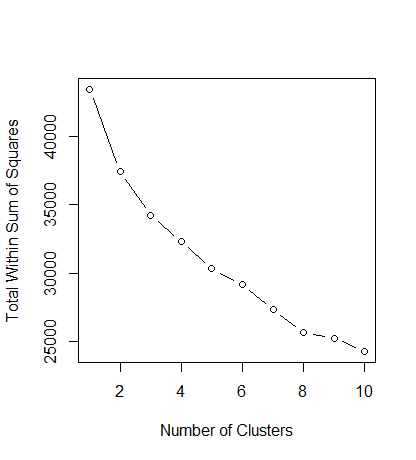
\includegraphics[width=0.8\textwidth]{unsupervised_figures/elbow_method_pca.png}
    \caption{Elbow Method Plot for Determining Optimal Number of Clusters}
    \label{fig:elbow_plot}
\end{figure}
    \item \textbf{Running K-Means Clustering:} With the optimal number of clusters (k = 8) determined, we proceeded to apply the K-Means clustering algorithm to our PCA-processed data. 

The final cluster assignments represented groupings of essays with similar characteristics as identified by the K-Means algorithm. 
    
    \item \textbf{Analyzing the Clusters:} After forming the clusters, their characteristics were analyzed. This included examining the average essay scores within each cluster, which provided insights into potential patterns or groupings in the essay scoring data.
\end{enumerate}

The results of K-Means clustering were expected to reveal natural groupings within the essays that could correlate with their scoring. These insights were intended to inform and enhance the development of subsequent supervised learning models.
\subsection{Clustering Algorithm 2: Hierarchical Clustering}
In addition to K-Means, Hierarchical Clustering was applied as a complementary approach. This method is particularly useful for identifying the hierarchical relationships between data points and does not require pre-specification of the number of clusters. 

\begin{enumerate}
    \item \textbf{Creating a Distance Matrix:} The first step involved calculating a distance matrix that represented the distances between each pair of points in our PCA-processed data. We used the Euclidean distance metric, which is a common choice for hierarchical clustering.

    \item \textbf{Building the Hierarchical Structure:} Using this distance matrix, a hierarchical clustering tree (dendrogram) was constructed. This was achieved using an agglomerative approach, where each data point initially represented a single-cluster, and pairs of clusters were merged as one moves up the hierarchy.

    \item \textbf{Merging Clusters:} In each successive iteration, the two nearest clusters were combined into a single cluster. The ‘nearest’ clusters were those with the smallest distance between them, which could be computed in various ways such as single linkage (minimum distance), complete linkage (maximum distance), or average linkage (average distance).

    \item \textbf{Creating the Dendrogram:} The process of merging continued iteratively, and at each step, the hierarchical clustering tree was updated. This tree, or dendrogram, visually represents the cluster formations and their respective proximities.

    \item \textbf{Determining the Number of Clusters:} To decide the number of clusters to retain, we examined the dendrogram and identified a level where the tree could be ‘cut’ to yield a meaningful clustering. It is difficult to determine the appropriate number of clusters \( k \) based on our dendrogram(figure 4), we introduce the Silhouette Analysis here.
\end{enumerate}
\begin{figure}[h]
    \centering
    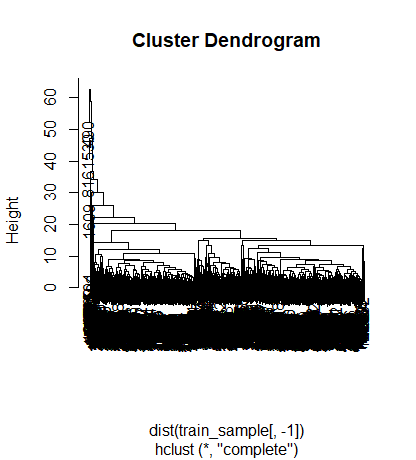
\includegraphics[width=0.8\textwidth]{unsupervised_figures/hclust_pca.png}
    \caption{Hierarchical Clustering Dendrogram}
    \label{fig:hierarchical_dendrogram}
\end{figure}
\paragraph{Determining Optimal Clusters with Silhouette Analysis}
We utilized silhouette analysis to objectively determine the optimal number of clusters \( k \). The silhouette method measures how similar an object is to its own cluster compared to other clusters. The silhouette score ranges from -1 to 1, where a high value indicates that the object is well matched to its own cluster and poorly matched to neighboring clusters.

The following steps were taken to implement silhouette analysis:

\begin{enumerate}
    \item \textbf{Computing Silhouette Scores:} For each value of \( k \), we computed the average silhouette score for all points. This was done using the \texttt{silhouette} function from the \texttt{cluster} package in R.
    
    \item \textbf{Iterating Over Various \( k \) Values:} We iterated over a range of \( k \) values and calculated the silhouette score for each. Typically, the range starts from 2 to an upper limit that makes sense for the dataset.
    
    \item \textbf{Selecting \( k \) with the Highest Score:} The optimal number of clusters \( k \) is the one that maximizes the average silhouette score. This indicates a structure where clusters are well separated and cohesive.
    
    \item \textbf{Visualizing the Results:} The silhouette scores for different \( k \) values were plotted, facilitating the selection of the number of clusters where the silhouette score starts to diminish.
\end{enumerate}

\begin{figure}[h]
    \centering
    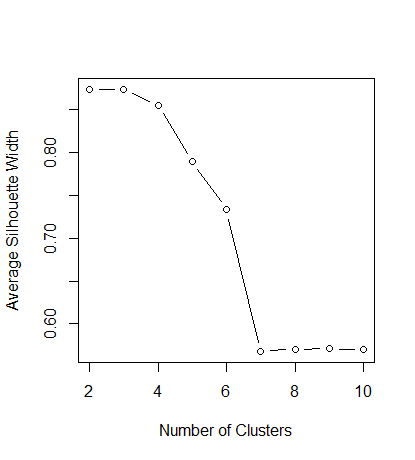
\includegraphics[width=0.8\textwidth]{unsupervised_figures/silhouette_method.png}
    \caption{Silhouette Analysis for Determining the Number of Clusters}
    \label{fig:silhouette_analysis}
\end{figure}

Following the silhouette analysis, we determined that the optimal number of clusters for our hierarchical clustering is \( k = 2 \). 

\subsection{Clustering Results}

The clustering algorithms provided insights into the natural groupings within the dataset. Below are the mean scores for each cluster as determined by K-Means and Hierarchical Clustering respectively.
\subsubsection{K-Means Clustering Results}
\begin{table}[H]
\centering
\begin{tabular}{cc}
\hline
\textbf{Cluster} & \textbf{Mean Score} \\
\hline
1 & 2.538462 \\
2 & 3.332000 \\
3 & 4.462898 \\
4 & 2.896514 \\
5 & 3.676056 \\
6 & 3.792683 \\
7 & 3.992678 \\
8 & 4.741860 \\
\hline
\end{tabular}
\caption{Mean scores for each cluster from K-Means Clustering.}
\label{table:hclust_scores}
\end{table}

\subsubsection{Hierarchical Clustering Results}
\begin{table}[H]
\centering
\begin{tabular}{cc}
\hline
\textbf{Cluster} & \textbf{Mean Score} \\
\hline
1 & 3.732405 \\
2 & 3.500000 \\
\hline
\end{tabular}
\caption{Mean scores for each cluster from K-Means Clustering.}
\label{table:kmeans_scores}
\end{table}

\subsubsection{Association with Outcome Variable}
The association between the clustering results and the outcome variable—in this case, the essay score—was evaluated. Using the K-Means and Hierarchical Clustering methods, it was possible to identify patterns that were related to the essay scores. There was a stratification effect visible in the mean scores within the clusters, with certain clusters having higher or lower essay scores. This implies that the clusters might be capturing underlying characteristics that are important for figuring out an essay's grade.

\subsubsection{Insights from Clustering Results}
The clustering results provide important information into the data structure and the relationships between different essays. Essays that belong to the same cluster, for example, may have similar topics, writing styles, or other latent characteristics that are important in the scoring process but are not measured directly. For the supervised learning models, these discoveries may direct future feature engineering and data preprocessing procedures.

\subsubsection{Utility for Supervised Model}
The clusters identified could be useful in enhancing the predictive power of the supervised models. By integrating cluster assignments as new features, the model can leverage the information about the groupings that emerged from the unsupervised learning phase. For example, the centroid of a cluster or the distance of an essay from the centroid could be a valuable predictor that captures the essence of each group. Moreover, understanding cluster characteristics can help in formulating new hypotheses about the scoring process and tailoring the models to better fit the complexity of the dataset.

\subsection{Conclusion}
The clustering results are indeed associated with the outcome variable, providing a non-trivial partitioning of the data that reflects the scoring pattern. By revealing the intrinsic structure within the essays, the unsupervised learning approach not only aids in understanding the dataset better but also offers a strategic direction for improving supervised learning algorithms. The use of cluster-based features could potentially increase the accuracy and interpretability of the predictive models.



\section{Regression/Classification Models}

\subsection{Regression Model 1: Linear Regression with ridge/lasso penalty}
Since we have learnt from the Kaggle discussion that the linear regression models are not really effective for this dataset, 
we consider a penalty and see if it leads to a good performance. 
We start with raw Ridge and LASSO regression models. Using the \texttt{glmnet} package with 10-fold cross validation, 
we get the $R^2 \approx 0.49$ for both Ridge and LASSO regression when predicting with \texttt{lambda.min}. 
This is not a good result, so we try the elastic net and lambda values for tuning. 
\paragraph{Elastic Net}
The elastic net is a combination of the Ridge and LASSO regression as shown in the lecture. 
The related tuning parameter is $\alpha$, which decides the proportion of the two penalties. 
In this setting, we iterate all $\alpha \in [0, 1]$ with 0.01 increments. 
In additional, we use the default lambda sequences for each $\alpha$. 
The tuning result is shown in \hyperref[fig:elastic_net]{Figure 3}.
\begin{figure}[H]
    \centering
    \includegraphics*[scale=0.25]{figures/elastic_net.png}
    \caption{Elastic Net: Tuning $\alpha$}
    \label{fig:elastic_net}
\end{figure}
It is clear that the LASSO penalty $\alpha = 1$ does not really help with the prediction.
The best $R^2$ is reached with the pure Ridge model. However, the difference is not significant, 
because of the fact that the linear assumption may not hold for this dataset.
\paragraph{Tuning Lambda}
The default lambda sequence may not be the best choice for our dataset.
Thus, we use a grid of lambda with exponential growth to find 
if a large penalty can influence the prediction. The lambda grid we use is 
\begin{align*}
    \texttt{lambda} = \texttt{exp(seq(-5, 5, 0.05))}
\end{align*}
The average tuning result with 100 simulations is shown in \hyperref[fig:lambda]{Figure 4}.
\begin{figure}[H]
    \centering
    \includegraphics*[scale=0.25]{figures/lambda.png}
    \caption{Ridge: Tuning $\lambda$}
\label{fig:lambda}
\end{figure}
Unexpectedly, the best $R^2$ is reached with the smallest lambda. 
It indicates that the Ridge penalty cannot help with the prediction, either. 
The interpretation of the bad fitting of linear regression model still lies in the absence of linear patterns in the data.
Even though Ridge penalty helps to resolve high multicollinearity and LASSO penalty 
helps to select features, they cannot help with the prediction without the linear assumption.

\subsection{Regression Model 2: Support Vector Regression}
Following the insights gained from the limited effectiveness of linear models, we explored Support Vector Regression (SVR) with the aim to capture non-linear patterns within the data. SVR is known for its robustness and effectiveness in handling non-linear relationships by using kernel functions. We utilized the \texttt{e1071} and \texttt{caret} packages in R for our implementation, with a radial basis function kernel, given its commonality in capturing a range of non-linear patterns.

\paragraph{SVR Tuning and Cross-Validation}
A grid search was conducted to tune two critical hyperparameters of SVR: the cost parameter $C$, which controls the trade-off between the model's complexity and the degree to which deviations larger than $\epsilon$ are tolerated in optimization; and $\sigma$, the kernel parameter which defines the width of the kernel function. We varied $C$ from $10^{-2}$ to $10^{2}$ and $\sigma$ from $10^{-3}$ to $10^{1}$ to find the optimal combination that minimizes the root mean squared error (RMSE).

\paragraph{Model Selection and Evaluation}
The model selection was based on 10-fold cross-validation, repeated three times to ensure the reliability of the evaluation. The best performing model, as indicated by the lowest RMSE, used a $\sigma$ value of 0.01 and $C$ value of 1. The corresponding R-squared value of approximately 0.5116232 suggests that SVR was able to explain over half of the variance in the essay scores, a substantial improvement over the linear models, yet it indicates room for further enhancement either through additional hyperparameter tuning or alternative modeling techniques.

The final selected SVR model, therefore, represents a step forward in predicting essay scores, highlighting the ability of kernel-based methods in capturing complex relationships within the data that are not necessarily linear.

Despite its improved performance, the SVR model still presents an R-squared value indicating that a portion of the variability in the essay scores remains unexplained, suggesting potential exploration into more nuanced features or alternative regression techniques that could further capture the intricacies of essay grading.

\subsection{Regression Model 3: LightBGM}
This model is inspired by ZhengHeng's method as presented in the literature review.
To recap the method, it is a gradient boosting framework that uses tree based algorithms. 
Upon many objectives, we choose the regression model. 
A raw fitting with default parameters yields an $R^2 \approx 0.55$. 
Then we choose to tune three parameters and check their effects on the prediction.
\begin{itemize}
    \item \texttt{n\_rounds}: the number of learnings iterations
    \item \texttt{learning\_rate}: the shrinkage rate, the default value is 0.1
    \item \texttt{num\_leaves}: maximal number of leaves inside a tree 
\end{itemize}
Since there are three parameters to tune, we fix a rather small grid for simplicity. 
\begin{align*}
    \texttt{nrounds = c(10, 20, 30)} \\
    \texttt{learning\_rate = c(0.1, 0.01, 0.001)} \\
    \texttt{num\_leaves = c(10, 20, 30)}
\end{align*}
\begin{figure}[H]
    \centering
    \includegraphics*[scale=0.25]{figures/rsquare_lightbgm.png}
    \caption{Ridge: Tuning lightbgm}
\label{fig:lightbgm}
\end{figure}
In \hyperref[fig:lambda]{Figure 5}, it can be observed that \texttt{num\_leaves} is a decidable 
paramter for the prediction, where the best $R^2 \approx 0.55$ was already given by the default value.
\texttt{learning\_rate}, on the other hand, would slightly affect the prediction: 
the accuracy $R^2$ increases slightly, as the learning rate decreases. While the other two 
paramters do have an influence, \texttt{nrounds} is not really effective here:
because a fast convergence of the predicion is easily witnessed.  

Different from what we have expected, the lightbgm model does not significantly rely on the computation power. 
Without using a GPU, we still manage to train and use the model in a reasonable time. 
Similarly, it did not yield an extraordinarily good result, either. Although the result is much better
than the classical regressors and classifierse, it is still not comparable to deep learning models 
that conquer the leaderboard.

\subsection{Classification Model: Random Forest}
For classification, we choose the random forest model using the R package \texttt{randomForest}.
The simple fitting using the default parameters gives us an \texttt{accuracy} of $\alpha = 0.3232$. 
Taking look at the confusion matrix, we found that prediction is concentrated along the diagonal, 
but does not have a high accuracy. So we present a new metric, \texttt{accuracy with tolerance}. 
This is the percentage of observations that are predicted within a tolerance $0.5$ of the true value.
\begin{align*}
    \tau = \texttt{Accuracy with tolerance} = \dfrac{\sum \texttt{diag} + \sum \texttt{subdiag} + \sum \texttt{superdiag}}{\sum \texttt{Observations}}
\end{align*}
In the simple fitting, $\tau = 0.7232$, which proves a good concentrtion of random forest model. 
\paragraph{Parameter Tuning}
The tuning goal of the model is to increase both the \texttt{accuracy} and the \texttt{accuracy with tolerance}.
Amongst many tuning parameters of random forest, we focus on \texttt{mtry} and \texttt{nodesize} with default 
\texttt{ntree} = 500. The grid we used is 
\begin{align*}
    \texttt{mtry} &\in \{1, 3, 5, 8, 10, 12, 15, 20, 25, 40,  50 \} \\
    \texttt{nodesize} &\in \{1, 3, 5, 8, 10, 12, 15, 20, 25, 40,  50 \}
\end{align*}
where the default values are $\texttt{mtry} = 5$ and $\texttt{nodesize} = 1$. 
The \hyperref[fig:contour]{contour plots} shows a best fit at $\texttt{mtry} \approx 11$ and $\texttt{nodesize} \approx 40$.
We may conclude that the effect of the random forest model is limited at $\alpha \approx 0.35$
and $\tau \approx 0.75$. Since there is an obvious concentration, 
this model is useful in the sense that it can show a general trend of the score.
However, it is not a good choice for sophisticated prediction as of the low accuracy.
\begin{figure}[H]
    \includegraphics*[scale=0.25]{figures/contour_plot_accuracy.png}
    \includegraphics*[scale=0.25]{figures/contour_plot_accuracy_with_tolerance.png}
    \caption{Contour plots of \texttt{accuracy} and \texttt{accuracy with tolerance}}
    \label{fig:contour}
\end{figure}

\paragraph{Variable Importance}
Another property of the random forest model is that it can provide a report on variable importance. 
A brief analysis and visualizatin of importance was already shown in \hyperref[fig:RF_important]{Variable Importance Based on Random Forest}.

\end{document}
